\documentclass[10pt,a4paper,onecolumn]{article}
\usepackage[latin1]{inputenc}
\usepackage{amsmath}
\usepackage{amsfonts}
\usepackage{amssymb}
\usepackage{makeidx}
\usepackage{graphicx}
\usepackage{url}
\usepackage{verbatim}
\usepackage{textcomp}
\usepackage{footnote}
\usepackage{hyperref}

\hypersetup{
    colorlinks,
    % citecolor=black,
    % filecolor=black,
    % linkcolor=black,
    % urlcolor=black
}

\begin{document}

\author{Yi Chen\\
   California institute of technology\\
   \texttt{chen.yi.first@gmail.com}}
\title{2.66 $pb^{-1}$ Z Candle Note Draft (pieces)}
\date{\today}
\maketitle

\tableofcontents
\clearpage 

\section{Introduction}

N/A.  I'll fill this in later.

\section{Data \& MC samples}

The monte-carlo simulations used in this note are summarized in table \ref{Table_MCSamples}.

\begin{table}[h]
   \caption{MC samples used.}
   \centering
   \begin{tabular}{|c|c|c|c|c|}
   \hline
   MC & Sample & Generator & Number of events \\\hline
   $Z\rightarrow\mu\mu$ + Jets & ??? & MADGRAPH & ??? \\\hline
   $W\rightarrow\mu\nu_\mu$ + Jets & ??? & MADGRAPH & ??? \\\hline
   $t\bar{t}$ + Jets & ??? & MADGRAPH & ??? \\\hline
   QCD (with two muons) & ??? & PYTHIA6 & ??? \\\hline
   \end{tabular}
   \label{Table_MCSamples}
\end{table}

Data samples included in this note are listed in table \ref{Table_DataSamples}.

\begin{table}[h]
   \caption{Data samples}
   \centering
   \begin{tabular}{|c|c|c|c|c|c|}
   \hline
   Run range & dataset & integrated luminosity \\\hline
   132440-191053 & /Run2010/GodDataSetForMuon & 1.069 $ab^{-1}$ \\\hline
   \end{tabular}
\end{table}

\section{Event cleaning}

Meow.

\section{Jet flavors}

All the jets are clustered using the anti-Kt algorithm with cone radius 0.5.  A few different types of jeta are considered in
this analysis.

\begin{enumerate}
\item Calorimetric jet (\emph{CaloJet}).  The jet constituents are taken from both hadronic calorimeter deposits and electomagnetic calorimeter deposits.
   The calorimeters are first combined into \emph{calotowers} according the the geometrical locations of the cells.
   Calotowers are then treated as four vector with zero norm to be included in the jet clustering algorithm.
   The jets need to be corrected for energy.  To estimate the effect of the energy correction, we also perform the analysis in terms of uncorrected energies.
   The threshold for counting CaloJets is 30 GeV/c, while the threshold for couting uncorrected CaloJets is 20 GeV/c.
\item Track jet.  All tracks that pass some basic quality selection criteria are served as input to the jet clustering algorithm, again treating them as massless.
   We require that the number of hits along the track is greater than 6, and the normalized $\chi^2$ is smaller than 20.
   The track vertex, compared to the primary vertex, has to be within 0.1cm in z direction, 0.1 cm in magnitude, and 600 $\mu$m in the transverse direction.
   Also, if there exists another reconstructed vertex that is closer to the best primary vertex, the track is not included in the jet clustering.
   The pseudorapidity of the track is required to be $-2.4 < |\eta| < 2.4$, and the momentum is required to be within range 0.5-500 GeV/c.
   The threshold for track jet counting is 20 GeV/c.
\item Particle flow jet (\emph{PF jet}).  There is an elaborate set of algorithms that attempts to reconstruct particle candidates as good as possible,
   and then to start physics analysis from there.  The jet algorithms take in the reconstructed candidates as input.
   The threshold for PF jet counting is 20 GeV/c.  Compatibility with the primary vertex is not implemented yet.
\end{enumerate}

\section{Selections.  Muon, Z.  Isolation}

In order to retain as much signal as possible, only a minimal selection is applied to data.
For candidate muons, we require the following.

\begin{enumerate}
\item The muon is reconstructed both as global muon and tracker muon
\item One valid pixel hit for the muon track is required to be present, and a total of 6 hits in the tracker system is required.
\item We also require that there is one valid hit in the muon chambers that is consistent with the global track.
\item The maximum allowed global muon track fitted $\chi^2$ is 10.
\item The PT threshold in this analysis for the first leg (tighter) muon is set to be 15 GeV/c with pseudorapidity range $-2.1 < |\eta| < 2.1$.
\item The limit on second leg muon is more relaxed for more statistics, and it is set on 10 GeV/c with range $-2.4 < |\eta| < 2.4$.
\end{enumerate}

An additional isolation requirement is required on both muons that make up the Z candidate.
This is mainly due to the fact that in the standard particle-flow jet clustering algorithm, the muons are considered as part
of the input collections to the clustering algorithm, and because of the high transverse momentum, the muons are clustered
as jets, as shown in figure \ref{Figure_CandidateMuonVsClosestJetEtaPhi}.  Furthermore, the muon jets tend to take up additional soft particles
in the vicinity of the muon (see figure \ref{Figure_CandidateMuonVsClosestJetPT}), causing extra systematics uncertainty in jet-counting.
Therefore, a isolation cut is selected as 30\% of relative combined isolation with cone size 0.3.  This causes roughly 5\%
efficiency drop for one-jet case, consistent with expectations, as shown in figure \ref{Figure_IsolationCutVsRejectionPercentage}.

\begin{figure}
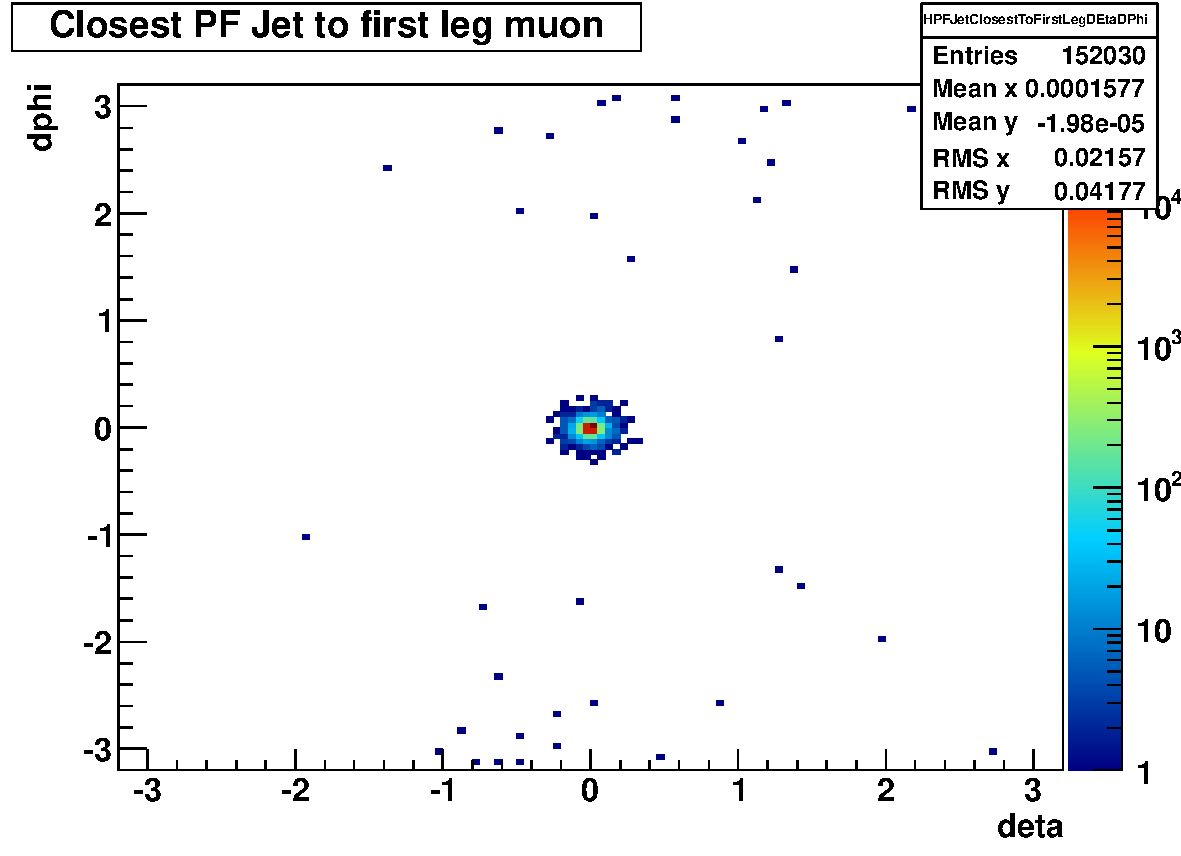
\includegraphics[width=110mm]{HPFJetClosestToFirstLegDEtaDPhi.pdf}
\caption{Candidate muon vs. closest jet, deta dphi plot (MC signal)}
\label{Figure_CandidateMuonVsClosestJetEtaPhi}
\end{figure}

\begin{figure}
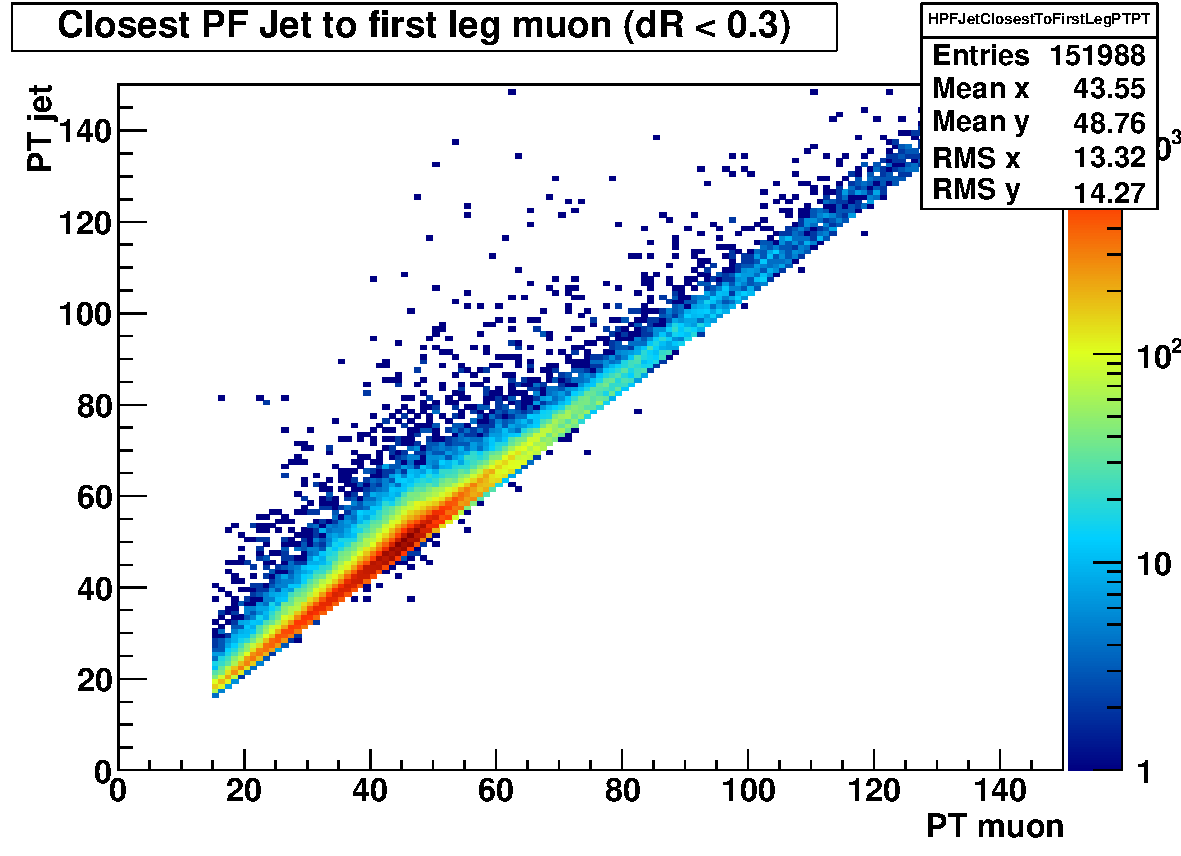
\includegraphics[width=110mm]{HPFJetClosestToFirstLegPTPT.pdf}
\caption{Muon PT vs. closest jet PT (MC signal)}
\label{Figure_CandidateMuonVsClosestJetPT}
\end{figure}

\begin{figure}
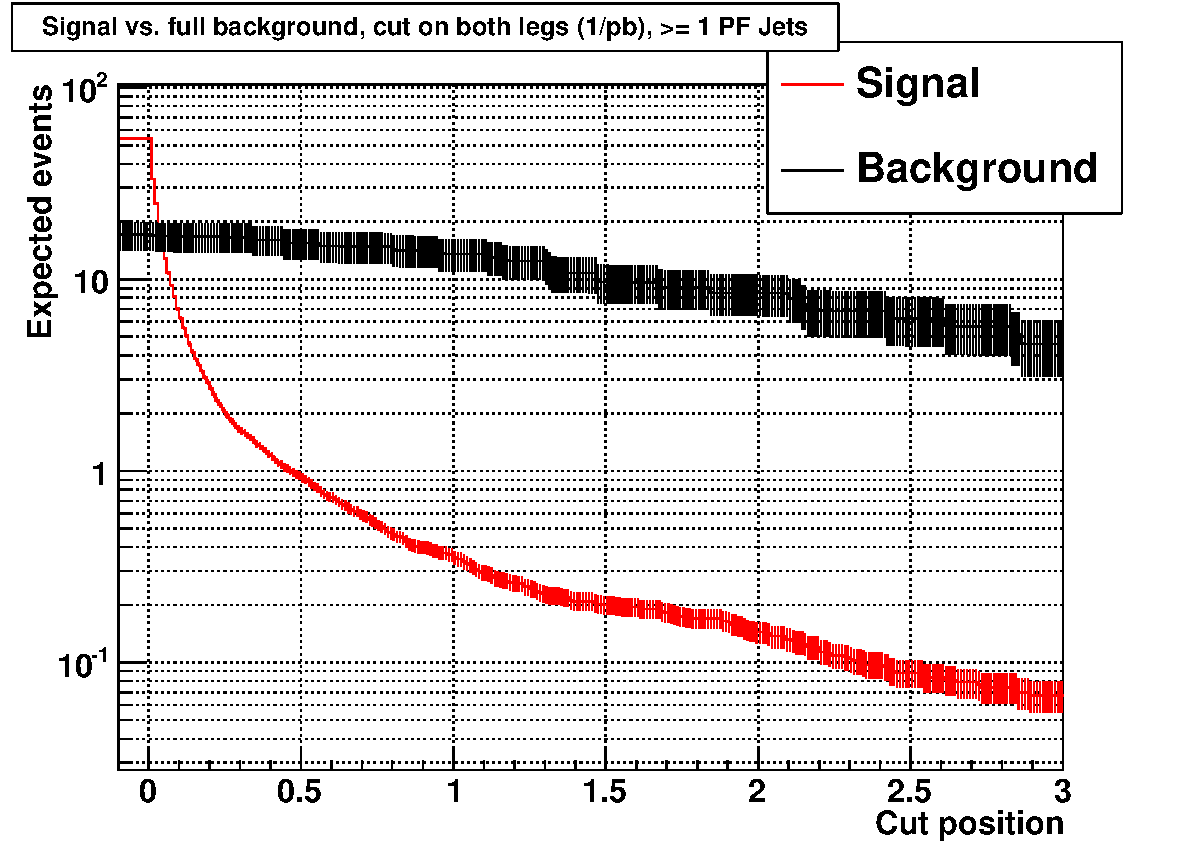
\includegraphics[width=110mm]{DoubleLeg_WithQCD_1PFJet.pdf}
\caption{Isolation cut vs. percentage that was cut out in MC signal events}
\label{Figure_IsolationCutVsRejectionPercentage}
\end{figure}

For any event with at least two good muon candidates as defined in the previous section, the muon pair is formed as a Z candidate if
the invariant mass of the two muons are with range 60-120 GeV/$c^2$.  An additional requirement to reject fake muon pairs is to require
that the two muons are at least 0.01 units apart in $\Delta R \equiv \sqrt{\Delta\eta^2 + \Delta\phi^2}$.

\section{MC sample efficiencies}

The efficiency of each step in the selection for MC samples are shown in table \ref{Table_MCSelectionEfficiency}.
In table \ref{Table_MCJetWiseSelectionEfficiencyCaloJet} we show the selection efficiency for different calorimetric jet counts.

\begin{table}[htdp]
 \caption{Selection efficiency for signal and background for each
    applied requirement. The values quoted are computed with respect
    to the previously-applied selection.\label{tab:effSel}}
 \centering
 \begin{tabular}{|c|c|c|c|c|}
   \hline
   \verb|Sample| & $Z+jets$ & $W+jets$ & $t \bar t+jets$ & $QCD$ \\
   \hline
   \verb|Two Muons|          & $ 57.78 \pm 0.16 $ & $ 4.38 \pm 0.01 $ & $ 30.53 \pm 0.06 $ & $ 57.84 \pm 0.09 $ \\
   \verb|Two Global Muons|   & $ 89.65 \pm 0.29 $ & $ 7.28 \pm 0.04 $ & $ 40.78 \pm 0.12 $ & $ 58.75 \pm 0.13 $ \\
   \verb|Pixel Hits|         & $ 99.45 \pm 0.33 $ & $ 92.99 \pm 0.76 $ & $ 97.46 \pm 0.35 $ & $ 95.63 \pm 0.23 $ \\
   \verb|Tracking Hits|      & $ 99.95 \pm 0.34 $ & $ 97.22 \pm 0.81$ & $ 98.94 \pm 0.36 $ & $ 99.11 \pm 0.24 $ \\
   \verb|Valid Muon Hits|    & $ 97.40 \pm 0.33 $ & $ 67.90 \pm 0.64 $ & $ 86.60 \pm 0.32 $ & $ 78.34 \pm 0.21 $ \\
   \verb|Muon |$\chi^2$      & $ 99.00 \pm 0.34 $ & $ 92.39 \pm 0.96 $ & $ 95.99 \pm 0.38 $ & $ 97.47 \pm 0.27 $ \\
   \verb|Isolation |         & $ 96.94 \pm 0.33 $ & $ 25.90 \pm 0.43$ & $ 14.49 \pm 0.11 $ & $ 28.56 \pm 0.12 $ \\
   $p_T$ \verb|and| $|\eta|$ & $ 91.67 \pm 0.33 $ & $ 0.55 \pm 0.11 $ & $ 32.99 \pm 0.49 $ & $ 0.00 \pm nan $ \\
   \hline
   \verb|Total|              & $ 44.12 \pm 0.14 $ & $ 0.00 \pm 0.00 $ & $ 0.48 \pm 0.01 $ & $ 0.00 \pm nan $ \\
   \hline
   \end{tabular}
\label{table}
\end{table}

\begin{table}[htdp]
   \caption{Expected number of events in (2.66 pb$^{-1}$ for signal and background Monte Carlo samples.\label{tab:effSel}}
       \centering
       \begin{tabular}{|c|c|c|c|c|}
       \hline
       \verb|Jet Counting| & $Z+jets$ & $W+jets$ & $t \bar t+jets$ & $QCD$ \\
       \hline
       \multicolumn{5}{|c|}{PFJets} \\
       \hline
       $N(\geq 0~jets)$       & $ 938.78 \pm 30.64 $ & $ 0.16 \pm 0.41 $ & $ 1.21 \pm 1.10 $ & $ 0.00 \pm 0.00 $ \\
       $N(\geq 1~jets)$       & $ 140.18 \pm 11.84 $ & $ 0.03 \pm 0.18 $ & $ 1.18 \pm 1.09 $ & $ 0.00 \pm 0.00 $ \\
       $N(\geq 2~jets)$       & $ 25.05 \pm 5.00 $ & $ 0.01 \pm 0.11 $ & $ 0.95 \pm 0.98 $ & $ 0.00 \pm 0.00 $ \\
       $N(\geq 3~jets)$       & $ 4.54 \pm 2.13 $ & $ 0.01 \pm 0.11 $ & $ 0.41 \pm 0.64 $ & $ 0.00 \pm 0.00 $ \\
       $N(\geq 4~jets)$       & $ 0.90 \pm 0.95 $ & $ 0.00 \pm 0.00 $ & $ 0.13 \pm 0.36 $ & $ 0.00 \pm 0.00 $ \\
       \hline
       \multicolumn{5}{|c|}{TrackJets} \\
       \hline
       $N(\geq 0~jets)$       & $ 938.78 \pm 30.64 $ & $ 0.16 \pm 0.41 $ & $ 1.21 \pm 1.10 $ & $ 0.00 \pm 0.00 $ \\
       $N(\geq 1~jets)$       & $ 99.29 \pm 9.96 $ & $ 0.03 \pm 0.18 $ & $ 1.08 \pm 1.04 $ & $ 0.00 \pm 0.00 $ \\
       $N(\geq 2~jets)$       & $ 13.90 \pm 3.73 $ & $ 0.01 \pm 0.11 $ & $ 0.67 \pm 0.82 $ & $ 0.00 \pm 0.00 $ \\
       $N(\geq 3~jets)$       & $ 2.24 \pm 1.50 $ & $ 0.00 \pm 0.00 $ & $ 0.22 \pm 0.47 $ & $ 0.00 \pm 0.00 $ \\
       $N(\geq 4~jets)$       & $ 0.35 \pm 0.59 $ & $ 0.00 \pm 0.00 $ & $ 0.06 \pm 0.24 $ & $ 0.00 \pm 0.00 $ \\
       \hline
       \multicolumn{5}{|c|}{CaloJets} \\
       \hline
       $N(\geq 0~jets)$       & $ 938.78 \pm 30.64 $ & $ 0.16 \pm 0.41 $ & $ 1.21 \pm 1.10 $ & $ 0.00 \pm 0.00 $ \\
       $N(\geq 1~jets)$       & $ 211.96 \pm 14.56 $ & $ 0.07 \pm 0.26 $ & $ 1.19 \pm 1.09 $ & $ 0.00 \pm 0.00 $ \\
       $N(\geq 2~jets)$       & $ 43.27 \pm 6.58 $ & $ 0.03 \pm 0.16 $ & $ 1.02 \pm 1.01 $ & $ 0.00 \pm 0.00 $ \\
       $N(\geq 3~jets)$       & $ 8.63 \pm 2.94 $ & $ 0.01 \pm 0.11 $ & $ 0.52 \pm 0.72 $ & $ 0.00 \pm 0.00 $ \\
       $N(\geq 4~jets)$       & $ 1.81 \pm 1.35 $ & $ 0.00 \pm 0.00 $ & $ 0.21 \pm 0.46 $ & $ 0.00 \pm 0.00 $ \\
       \hline
       \multicolumn{5}{|c|}{UncorrectedCaloJets} \\
       \hline
       $N(\geq 0~jets)$       & $ 938.78 \pm 30.64 $ & $ 0.16 \pm 0.41 $ & $ 1.21 \pm 1.10 $ & $ 0.00 \pm 0.00 $ \\
       $N(\geq 1~jets)$       & $ 114.41 \pm 10.70 $ & $ 0.05 \pm 0.21 $ & $ 1.15 \pm 1.07 $ & $ 0.00 \pm 0.00 $ \\
       $N(\geq 2~jets)$       & $ 17.73 \pm 4.21 $ & $ 0.01 \pm 0.08 $ & $ 0.81 \pm 0.90 $ & $ 0.00 \pm 0.00 $ \\
       $N(\geq 3~jets)$       & $ 2.99 \pm 1.73 $ & $ 0.01 \pm 0.08 $ & $ 0.30 \pm 0.55 $ & $ 0.00 \pm 0.00 $ \\
       $N(\geq 4~jets)$       & $ 0.59 \pm 0.77 $ & $ 0.00 \pm 0.00 $ & $ 0.08 \pm 0.29 $ & $ 0.00 \pm 0.00 $ \\
       \hline
       \end{tabular}
\label{table}
\end{table}


\begin{table}[htdp]
 \caption{Selection efficiency for signal in different calo jet bin for each
    applied requirement. The values quoted are computed with respect
    to the previously-applied selection.}
 \centering
 \begin{tabular}{|c|c|c|c|c|c|}
   \hline
   \verb|Jet count| & $\ge 0 jets$ & $\ge 1 jet$ & $\ge 2 jets$ & $\ge 3 jets$ & $\ge 4 jets$ \\
   \hline
   \verb|Two Muons|          & $ 57.78 \pm 0.16 $ & $ 69.94 \pm 0.41 $ & $ 75.71 \pm 0.98 $ & $ 79.17 \pm 2.29 $ & $ 80.14 \pm 4.99 $ \\
   \verb|Two Global Muons|   & $ 89.65 \pm 0.29 $ & $ 89.98 \pm 0.59 $ & $ 89.59 \pm 1.27 $ & $ 89.95 \pm 2.83 $ & $ 88.36 \pm 5.99 $ \\
   \verb|Pixel Hits|         & $ 99.45 \pm 0.33 $ & $ 99.38 \pm 0.67 $ & $ 99.43 \pm 1.45 $ & $ 99.38 \pm 3.21 $ & $ 99.27 \pm 6.95 $ \\
   \verb|Tracking Hits|      & $ 99.95 \pm 0.34 $ & $ 99.95 \pm 0.67$ & $ 99.93 \pm 1.46 $ & $ 99.84 \pm 3.23 $ & $ 100.00 \pm 7.01 $ \\
   \verb|Valid Muon Hits|    & $ 97.40 \pm 0.33 $ & $ 97.05 \pm 0.66 $ & $ 97.06 \pm 1.43 $ & $ 97.17 \pm 3.17 $ & $ 95.82 \pm 6.79 $ \\
   \verb|Muon |$\chi^2$      & $ 99.00 \pm 0.34 $ & $ 98.77 \pm 0.68 $ & $ 98.66 \pm 1.47 $ & $ 98.38 \pm 3.24 $ & $ 98.46 \pm 7.08 $ \\
   \verb|Isolation |         & $ 96.94 \pm 0.33 $ & $ 90.77 \pm 0.64$ & $ 88.05 \pm 1.36 $ & $ 85.16 \pm 2.94 $ & $ 84.38 \pm 6.36 $ \\
   $p_T$ \verb|and| $|\eta|$ & $ 91.67 \pm 0.33 $ & $ 89.06 \pm 0.66 $ & $ 88.56 \pm 1.45 $ & $ 89.90 \pm 3.31 $ & $ 90.43 \pm 7.29 $ \\
   \hline
   \verb|Total|              & $ 44.12 \pm 0.14 $ & $ 48.44 \pm 0.32 $ & $ 50.32 \pm 0.74 $ & $ 51.72 \pm 1.70 $ & $ 50.60 \pm 3.63 $ \\
   \hline
   \end{tabular}
\label{table}
\end{table}


\begin{table}[htdp]
 \caption{Selection efficiency for signal in different uncorrected calo jet bin for each
    applied requirement. The values quoted are computed with respect
    to the previously-applied selection.}
 \centering
 \begin{tabular}{|c|c|c|c|c|c|}
   \hline
   \verb|Jet count| & $\ge 0 jets$ & $\ge 1 jet$ & $\ge 2 jets$ & $\ge 3 jets$ & $\ge 4 jets$ \\
   \hline
   \verb|Two Muons|          & $ 57.78 \pm 0.16 $ & $ 71.88 \pm 0.57 $ & $ 77.08 \pm 1.55 $ & $ 80.94 \pm 4.09 $ & $ 81.76 \pm 9.35 $ \\
   \verb|Two Global Muons|   & $ 89.65 \pm 0.29 $ & $ 89.93 \pm 0.78 $ & $ 89.42 \pm 1.97 $ & $ 89.42 \pm 4.89 $ & $ 89.21 \pm 11.02 $ \\
   \verb|Pixel Hits|         & $ 99.45 \pm 0.33 $ & $ 99.38 \pm 0.89 $ & $ 99.36 \pm 2.25 $ & $ 99.37 \pm 5.59 $ & $ 100.00 \pm 12.70 $ \\
   \verb|Tracking Hits|      & $ 99.95 \pm 0.34 $ & $ 99.96 \pm 0.90$ & $ 99.90 \pm 2.27 $ & $ 99.84 \pm 5.63 $ & $ 100.00 \pm 12.70 $ \\
   \verb|Valid Muon Hits|    & $ 97.40 \pm 0.33 $ & $ 96.77 \pm 0.88 $ & $ 97.01 \pm 2.22 $ & $ 97.46 \pm 5.53 $ & $ 96.77 \pm 12.39 $ \\
   \verb|Muon |$\chi^2$      & $ 99.00 \pm 0.34 $ & $ 98.59 \pm 0.90 $ & $ 98.57 \pm 2.28 $ & $ 99.02 \pm 5.67 $ & $ 100.00 \pm 12.91 $ \\
   \verb|Isolation |         & $ 96.94 \pm 0.33 $ & $ 89.80 \pm 0.85$ & $ 87.11 \pm 2.09 $ & $ 86.66 \pm 5.16 $ & $ 86.67 \pm 11.61 $ \\
   $p_T$ \verb|and| $|\eta|$ & $ 91.67 \pm 0.33 $ & $ 87.02 \pm 0.87 $ & $ 88.69 \pm 2.27 $ & $ 92.21 \pm 5.80 $ & $ 91.35 \pm 12.96 $ \\
   \hline
   \verb|Total|              & $ 44.12 \pm 0.14 $ & $ 47.87 \pm 0.43 $ & $ 50.55 \pm 1.16 $ & $ 55.37 \pm 3.13 $ & $ 55.88 \pm 7.16 $ \\
   \hline
   \end{tabular}
\label{table}
\end{table}


\section{Signal extraction (fit strategy)}

In order to extract signal yields from data, a fit is performed on the dimuon mass spectrum.
The signal shape is taken as the Cruijff function, defined as

\begin{equation}
f(M_{ll}; m, \sigma_L, \sigma_R, \alpha_L, \alpha_R) = N_s e^{-\dfrac{(M_{ll} - m)^2}{2 \sigma^2 + \alpha^2 (M_{ll} - m)^2}},\nonumber
\end{equation}

where $\sigma = \sigma_L (\sigma_R)$ for $M_{ll} < m (M_{ll} > m)$ and $\alpha = \alpha_L (\alpha_R)$ for $M_{ll} < m (M_{ll} > m)$.
The background shape is chosen as a falling exponential, as can be seen in the QCD sample which dominates the background in low
jet multiplicity bin.  When the number of jets is larger, events with $t\bar{t}$ start to have a significant contribution, and those are
also well-modeled by a falling exponential.
Even though the exponent is not the same in different samples, the exponent is floated in the fit, and the difference in exponent will be taken account for.

A minimum likelihood fit is performed simulatneously for all different jet counts, with the total likelihood written as

\begin{eqnarray}
L = (Prefactor) \times \displaystyle\sum_i \{ \displaystyle\sum_{n_{jet}=1}^{n_{max} - 1} \left( (N_{S, n_{jet}} - N_{S, n_{jet} + 1}) F_S(M_{ll}^i) + N_{B, n_{jet}} F_{B, n_{jet}}(M_{ll}^i) \right)
\delta_{n_{jet}, n_{jet}^i}\nonumber\\
+ \left( N_{S, n_{max}} F_S(M_{ll}^i) + N_{B, n_{max}} F_{B, n_{max}}(M_{ll}^i) \right) \theta(n_{jet}^i - n_{max}) \},
\nonumber
\end{eqnarray}

where $F_S$ is the signal PDF, constrained to be the same for all jet bins.  The background PDF, $F_{B, n_{jet}}$, is not constrained to
be the same for different jet bins, and the exponents are left floating in the fit.  Each term (except the last) is constrained to be with the same exclusive jet bin
through the Kronecker delta function $\delta_{n_{jet}, n_{jet}^i}$.
The last jet bin is inclusive, including all number of jets greater or equal to $n_{max}$, constrained by the step function $\theta(n_{jet}^i - n_{max})$.

All the parameters for signal PDF are floated except $\alpha_L$.  Since the $\alpha_L (\alpha_R)$ controls how large the tail is, if $\alpha_L$ is floated,
in the presense of background events, which is approximated by an exponential function, the tail of the signal PDF will be larger then real signal shape.
As a result, the signal yield will include significant contributions from background events, which does not serve our purpose of extracting the signal yield.
Fortunately, the signal shape does not depend too much on isolation, as shown in figure \ref{Figure_SignalShapeVsIsolation} in MC studies.
Therefore we can apply a very tight isolation cut to remove all backgrounds and some signal events, and fit to get $\alpha_L$ to be used to extract signal yield
as a function of jet multiplicity.

\begin{figure}
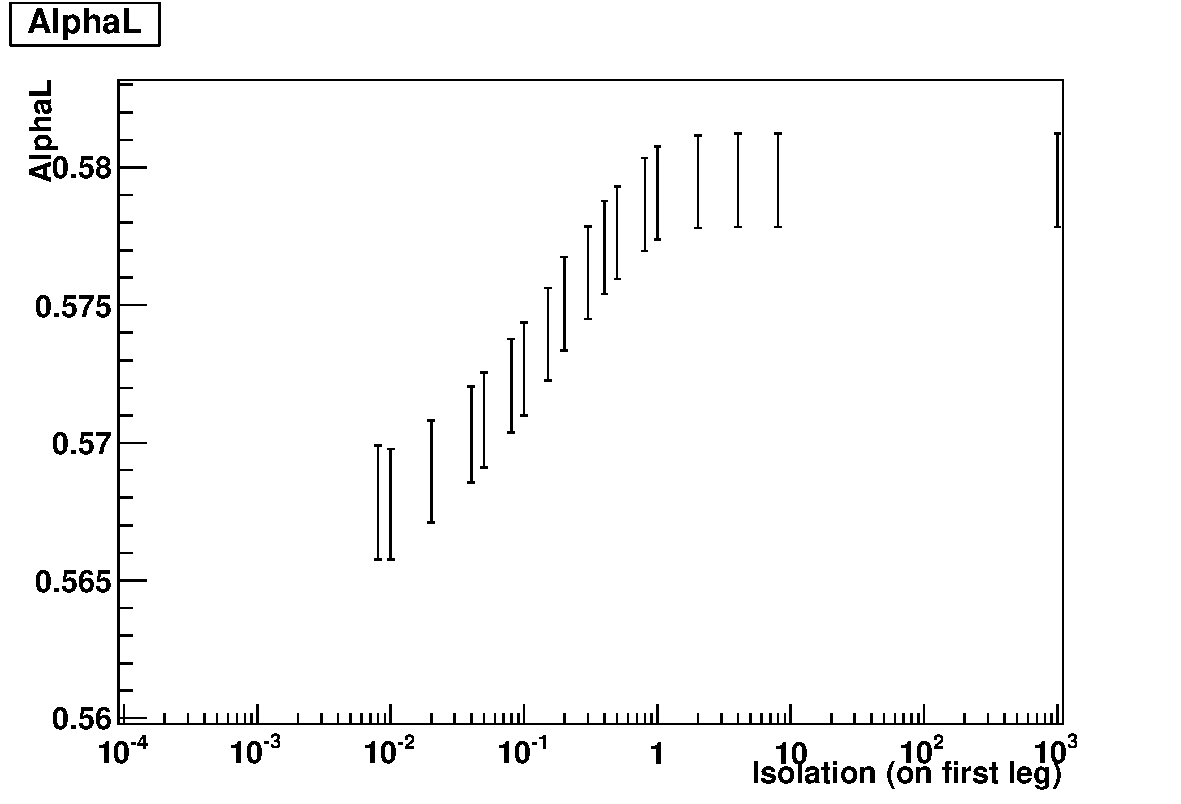
\includegraphics[width=110mm]{AlphaLVsIsolation_ReasonableIsolation.pdf}
\caption{Signal shape vs. isolation}
\label{Figure_SignalShapeVsIsolation}
\end{figure}

\section{Fit result on data}

The fit strategy described above is applied to data.  Fixed parameter $\alpha_L$ for each jet flavor is extracted separately, and the result is listed in table \ref{Table_DataAlphaL}.
After fitting, the extracted yields are shown in table \ref{Table_DataExtractedYields}, while the $N/(N+1)$ jet ratio is summarized in figures \ref{Figure_RatioFromDataCaloJet},
\ref{Figure_RatioFromDataUncorrectedCaloJet}, \ref{Figure_RatioFromDataPFJet} and \ref{Figure_RatioFromDataTrackJet}.

\begin{table}
\caption{Shape parameters for different jet flavors fitting to data with tight isolation cut}
\centering
   \begin{tabular}{|c|c|c|c|c|c|}
      \hline
      & CaloJet & Uncorrected CaloJet & PF Jet & Track jet \\\hline
      $m$ & 90.75 $\pm$ 0.39 & 91.27 $\pm$ 0.37 & 90.87 $\pm$ 0.37 & 90.79 $\pm$ 0.42 \\\hline
      $\alpha_L$ & 0.530 $\pm$ 0.013 & 0.494 $\pm$ 0.017 & 0.502 $\pm$ 0.015 & 0.529 $\pm$ 0.017 \\\hline
      $\alpha_R$ & 0.433 $\pm$ 0.016 & 0.458 $\pm$ 0.018 & 0.441 $\pm$ 0.018 & 0.416 $\pm$ 0.024 \\\hline
      $\sigma_L$ & 1.894 $\pm$ 0.280 & 2.514 $\pm$ 0.318 & 2.225 $\pm$ 0.292 & 1.895 $\pm$ 0.331 \\\hline
      $\sigma_R$ & 2.221 $\pm$ 0.255 & 1.840 $\pm$ 0.255 & 2.182 $\pm$ 0.265 & 2.378 $\pm$ 0.316 \\\hline
   \end{tabular}
   \label{Table_DataAlphaL}
\end{table}

\begin{table}
\caption{Data extracted yields}
\centering
   \begin{tabular}{|c|c|c|c|c|}
      \hline
      & CaloJet & Uncorrected CaloJet & PF Jet & Track jet \\\hline
      $N \ge 1$ & 799 $\pm$ 105 & 554 $\pm$ 26 & 681 $\pm$ 31 & 465 $\pm$ 22 \\\hline
      $N \ge 2$ & 166 $\pm$ 29 & 91 $\pm$ 11 & 141 $\pm$ 14 & 75 $\pm$ 10 \\\hline
      $N \ge 3$ & 26 $\pm$ 8 & 11 $\pm$ 5 & 25 $\pm$ 6 & 9 $\pm$ 3 \\\hline
      $N \ge 4$ & 6 $\pm$ 4 & 3 $\pm$ 3 & 3 $\pm$ 2 & 0 $\pm$ 2 \\\hline
   \end{tabular}
   \label{Table_DataExtractedYields}
\end{table}

\begin{figure}
   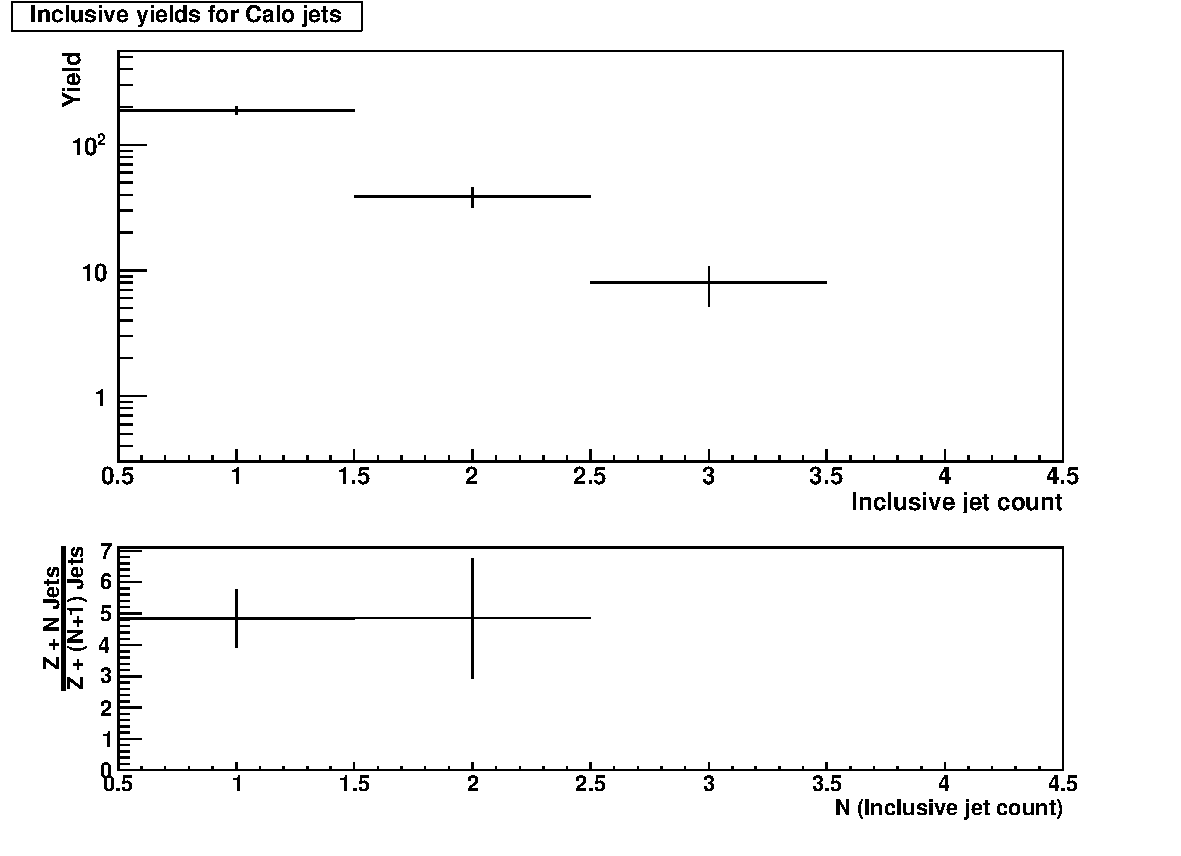
\includegraphics[width=110mm]{FinalPlot_FloatAll_Calo.pdf}
   \caption{Summary of N/(N+1) jet ratio for different kinds of jets}
   \label{Figure_RatioFromDataCaloJet}
\end{figure}

\begin{figure}
   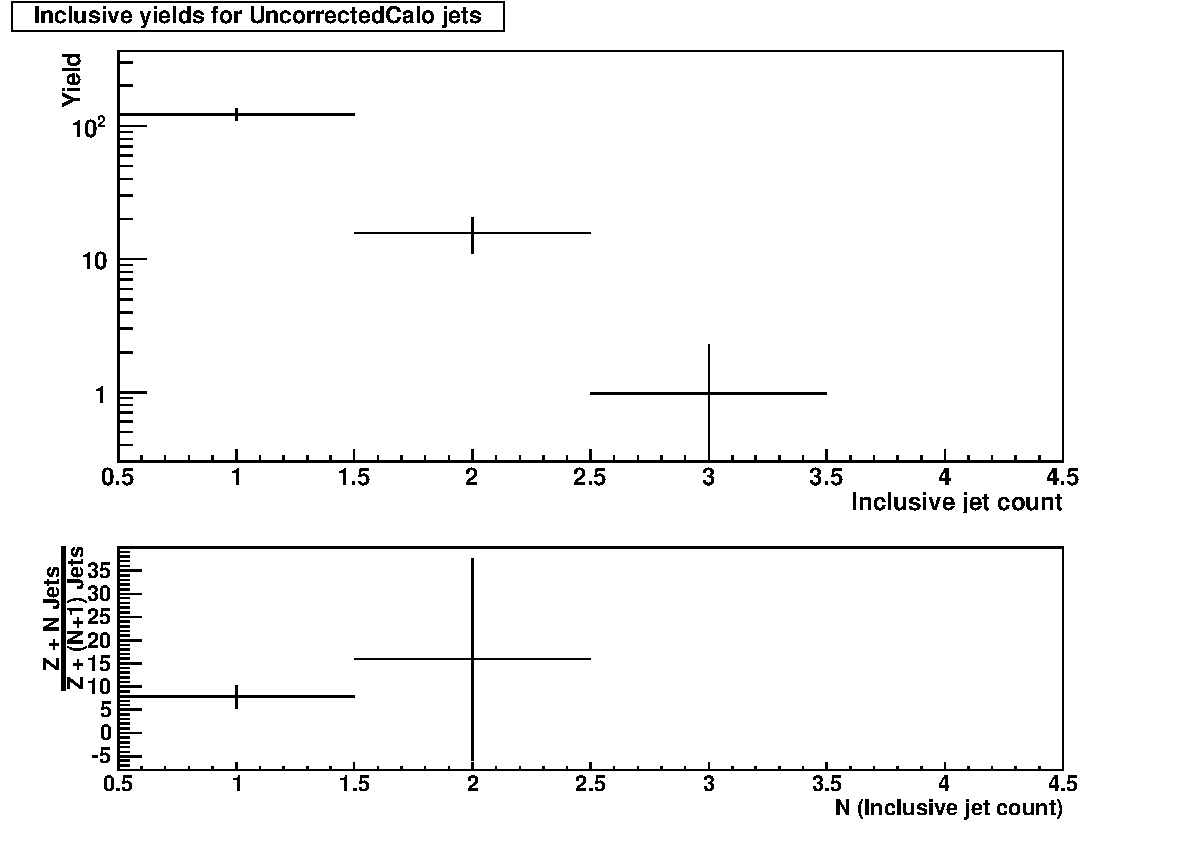
\includegraphics[width=110mm]{FinalPlot_FloatAll_UncorrectedCalo.pdf}
   \caption{Summary of N/(N+1) jet ratio for different kinds of jets}
   \label{Figure_RatioFromDataUncorrectedCaloJet}
\end{figure}

\begin{figure}
   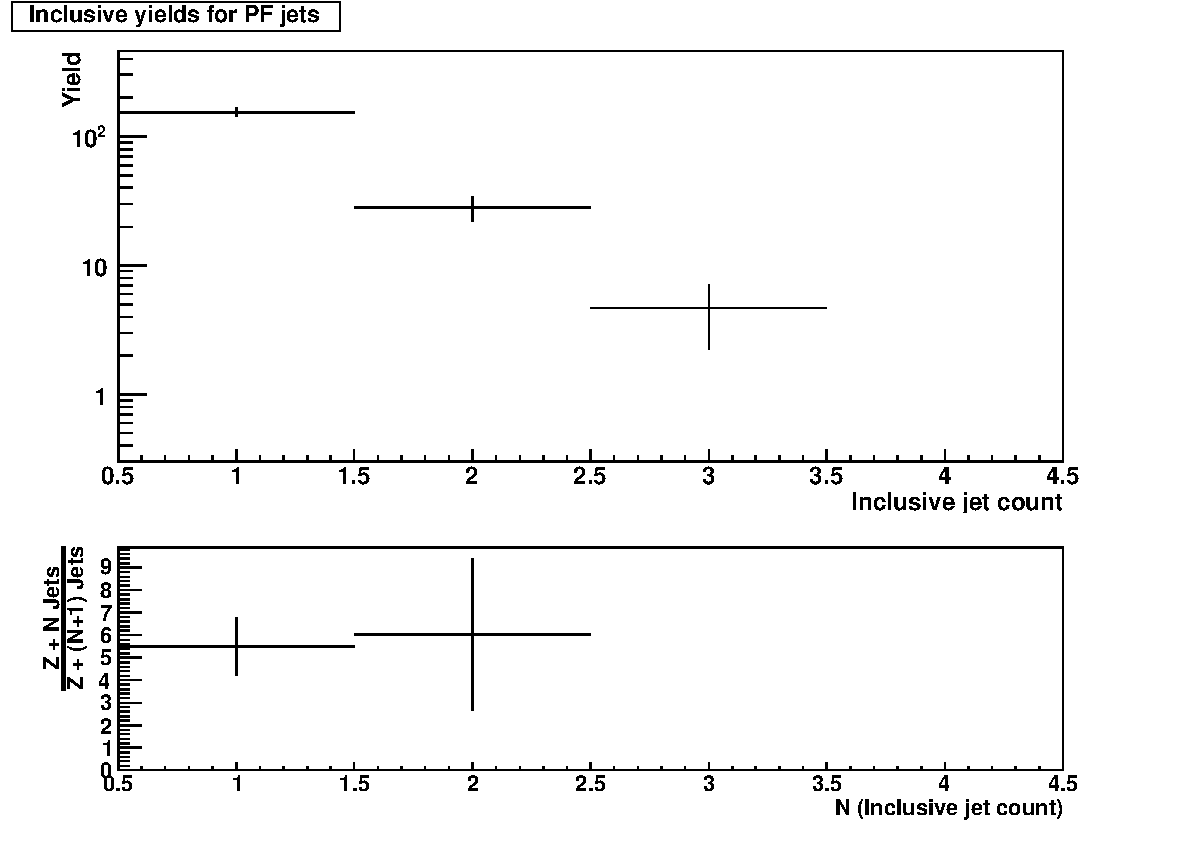
\includegraphics[width=110mm]{FinalPlot_FloatAll_PF.pdf}
   \caption{Summary of N/(N+1) jet ratio for different kinds of jets}
   \label{Figure_RatioFromDataPFJet}
\end{figure}

\begin{figure}
   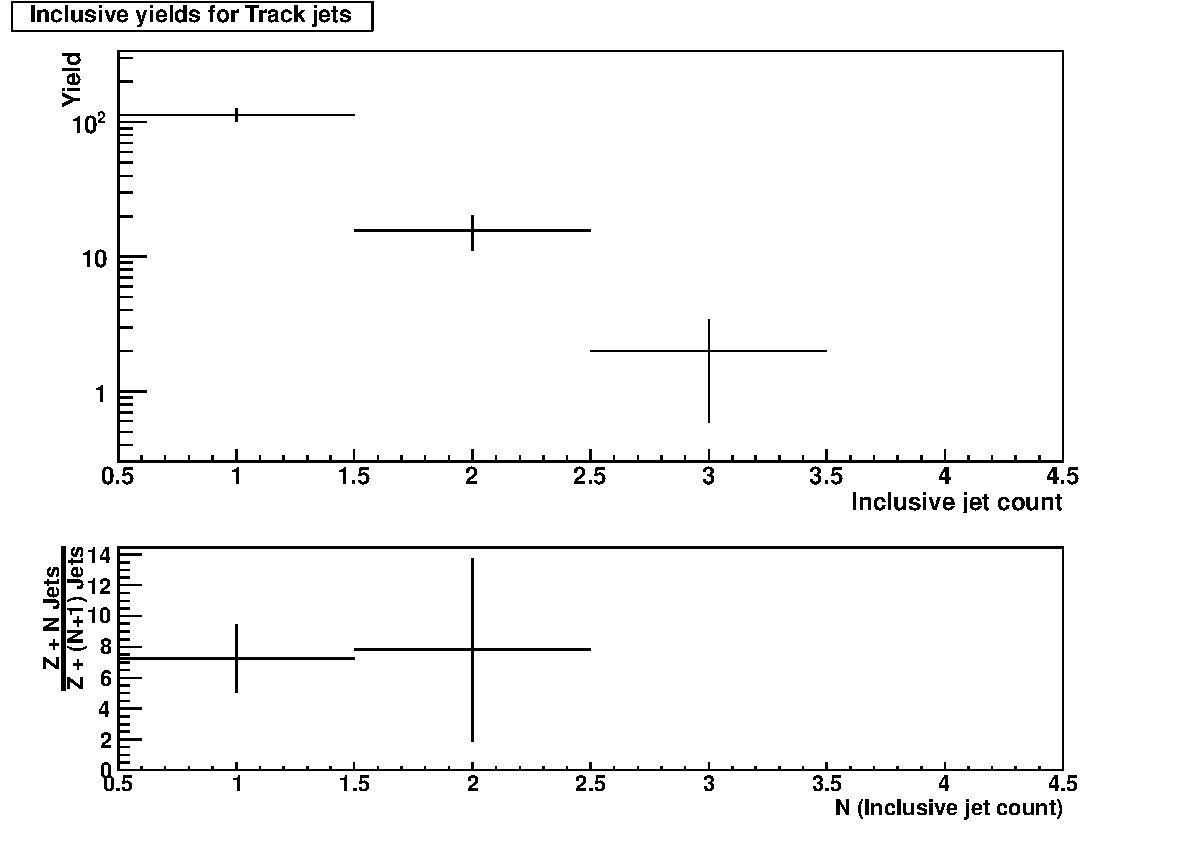
\includegraphics[width=110mm]{FinalPlot_FloatAll_Track.pdf}
   \caption{Summary of N/(N+1) jet ratio for different kinds of jets}
   \label{Figure_RatioFromDataTrackJet}
\end{figure}


\section{Toy studies: shape, parameters}

In order to demonstrate the dependence of each parameter in the signal fit, a toy study is performed.
The fitted Z signal shape is taken as a template, and 1000 toy experiment samples are generated assuming 50/pb of integrated luminosity.
Each toy experiment is then fitted with signal functional form with slightly different parameters compared to the input parameters.
The pull distribution of the signal yield is plotted and compared to Gaussian of width 1.

For each shape parameter, we vary it by -10\%, -5\%, -2.5\%, -1\%, 0\%, 1\%, 2.5\%, 5\% and 10\% while keeping other parameters fixed at the right (input) value.
The signal yield relative to perfect case is plotted in figures \ref{Figure_RelativeYieldChangingAlphaLOnly}, \ref{Figure_RelativeYieldChangingAlphaROnly},
\ref{Figure_RelativeYieldChangingSigmaLOnly} and \ref{Figure_RelativeYieldChangingSigmaROnly}.
We can see that the signal yield is most sensitive to $\alpha_L$ and neglegible in other parameters.
This is because of the radiation effects of the muons lower the mass, and naturally there will be a tail in the lower side of the peak.
Biases arise in estimating the size of the tail.
However, even in the case of $\alpha_L$, the bias in the signal yield is mild.

Fit with wrong $\alpha_L$ value while floating others is also analyzed with toy experiments.
This is an estimate of the bias in realistic conditions as in the fit to extract signal value.
The result is shown in figure \ref{Figure_RelativeYieldChangingAlphaLFloatingOthers}.
TODO: INSERT RESULT!

\begin{figure}

\includegraphics[width=110mm]{ToBeDrawn.pdf}
\caption{Signal yields relative to the perfect case when $\alpha_L$ is varied while keeping others fixed.}
\label{Figure_RelativeYieldChangingAlphaLOnly}
\end{figure}

\begin{figure}

\includegraphics[width=110mm]{ToBeDrawn.pdf}
\caption{Signal yields relative to the perfect case when $\alpha_R$ is varied while keeping others fixed.}
\label{Figure_RelativeYieldChangingAlphaROnly}
\end{figure}

\begin{figure}

\includegraphics[width=110mm]{ToBeDrawn.pdf}
\caption{Signal yields relative to the perfect case when $\sigma_L$ is varied while keeping others fixed.}
\label{Figure_RelativeYieldChangingSigmaLOnly}
\end{figure}

\begin{figure}

\includegraphics[width=110mm]{ToBeDrawn.pdf}
\caption{Signal yields relative to the perfect case when $\sigma_L$ is varied while keeping others fixed.}
\label{Figure_RelativeYieldChangingSigmaROnly}
\end{figure}

\begin{figure}

\includegraphics[width=110mm]{ToBeDrawn.pdf}
\caption{Signal yields relative to the perfect case when $\sigma_L$ is varied and floating others.}
\label{Figure_RelativeYieldChangingAlphaLFloatingOthers}
\end{figure}


\section{JES uncertainty}

Since CaloJets and PF jets are corrected for energy, there will be systematic uncertainties associated with the corrections.
The CMS-official numbers for the uncertainties is quoted as

\begin{enumerate}
\item 10\% overall scale for CaloJets
\item 5\% overall scale for PF jets
\item 2\% eta-dependent scale ($2\% \times |\eta|$) for both types of jets.
\item The two types of errors (absolute and eta-dependent) are assumed to be independent to each other.
\end{enumerate}

Therefore the strategy to estimate the systematics of the uncertainties is to perform the fit and extract signal yields for different jet multiplicities 4 additional times with different thresholds:

\begin{enumerate}
\item Original threshold + $10\%$
\item Original threshold - $10\%$
\item Original threshold + $2\% \times |\eta|$
\item Original threshold - $2\% \times |\eta|$
\end{enumerate}

The difference between different thresholds are taken as an estimate to the jet energy correction uncertainty.
The result, when applied to data, is shown in figures \ref{Figure_CaloJetJES} and \ref{Figure_PFJetJES} for CaloJets and PF jets respectively.

\begin{figure}
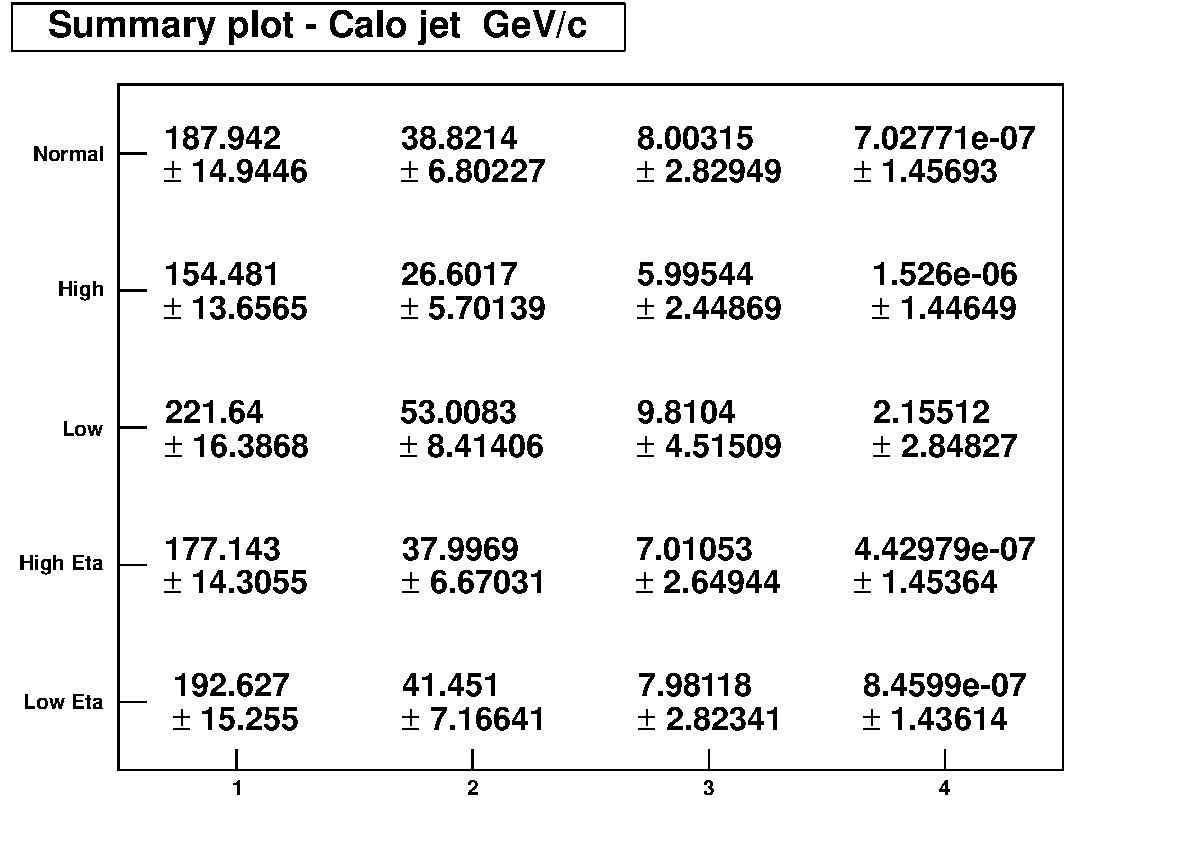
\includegraphics[width=110mm]{CaloJet_JES.pdf}
\caption{Jet energy scale uncertainty estimation for CaloJets}
\label{Figure_CaloJetJES}
\end{figure}

\begin{figure}
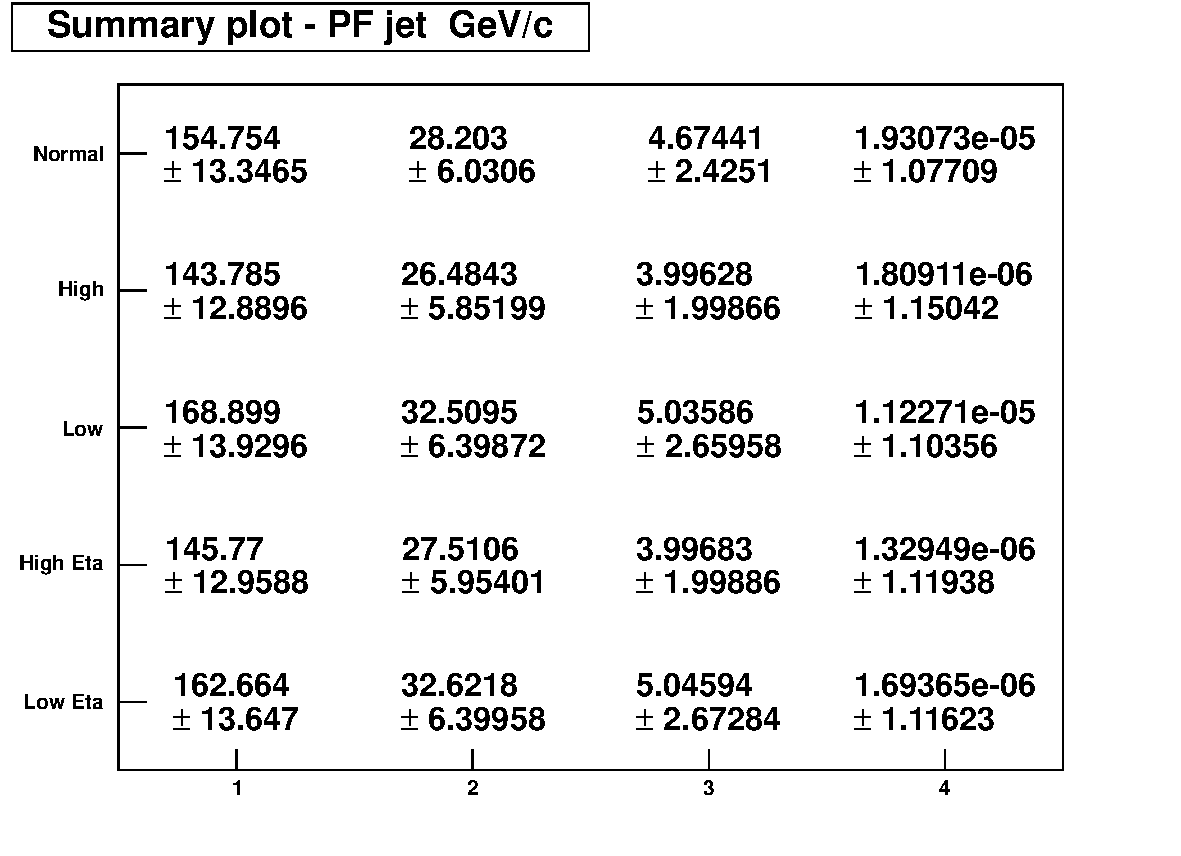
\includegraphics[width=110mm]{PFJet_JES.pdf}
\caption{Jet energy scale uncertainty estimation for PF jets}
\label{Figure_PFJetJES}
\end{figure}


\section{Anti-muon control sample}

To justify the choice of exponential PDF for background events, an anti-muon control sample check is performed.
This is done by comparing the following

\begin{enumerate}
\item MC QCD sample, normal selection
\item MC QCD sample, inverting isolation on the first leg muon
\item Data, inverting isolation on the first leg muon
\end{enumerate}

The result is shown in figure \ref{Figure_AntiMuonSingleLeg}.  Each histogram is scaled to the same area so that we can compare the shape.
Indeed, the shapes are similar to each other.  Unfortunately there isn't enough statistics on the QCD sample to accomodate the increasing statistics in data.

\begin{figure}
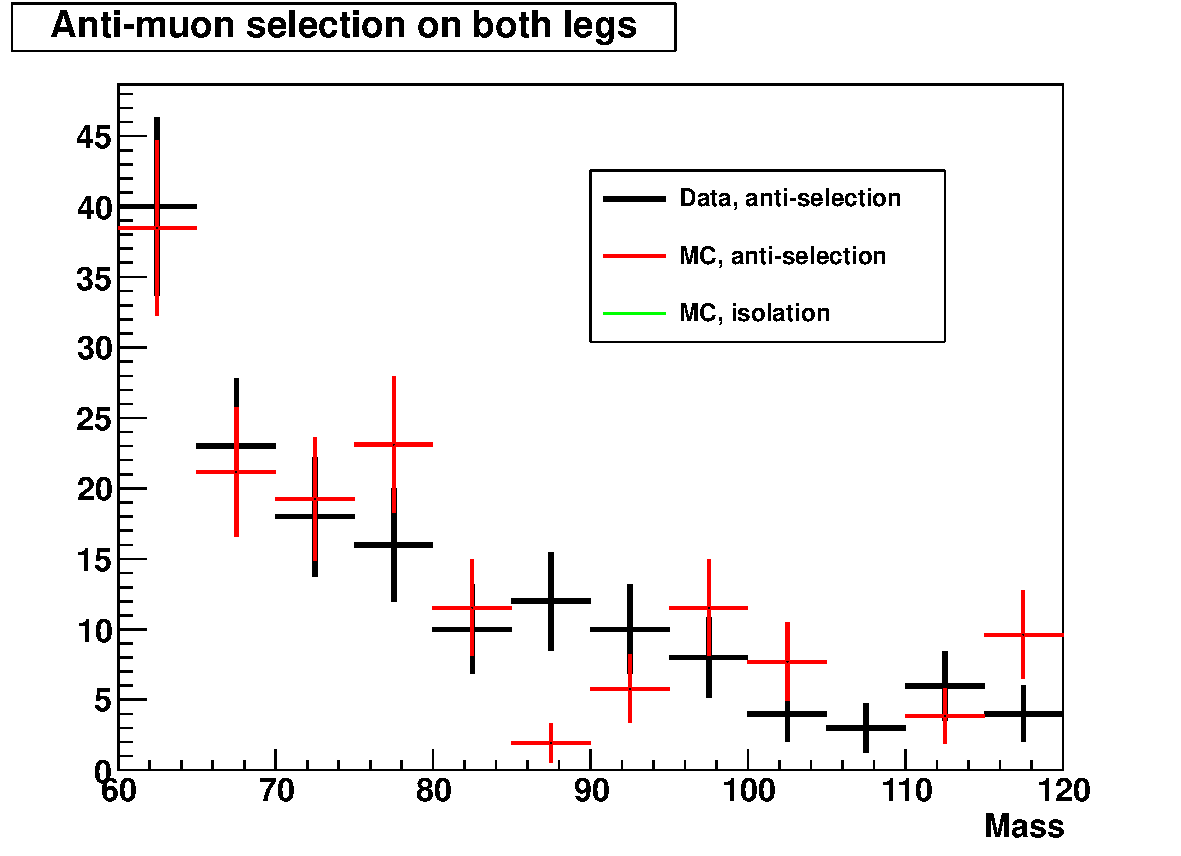
\includegraphics[width=110mm]{DoubleLegAntiMuon.pdf}
\caption{Anti-muon check}
\label{Figure_AntiMuonSingleLeg}
\end{figure}

\end{document}




